%%%%%%%%%%%%%%%%%%%%%%%%%%%%%%%%%%%%%%%%%
%
% (c) 2023 by Jennifer Laaser
%
% This work is licensed under the Creative Commons Attribution-NonCommercial-ShareAlike 4.0 International License. To view a copy of this license, visit http://creativecommons.org/licenses/by-nc-sa/4.0/ or send a letter to Creative Commons, PO Box 1866, Mountain View, CA 94042, USA.
%
% The current source for these materials is accessible on Github: https://github.com/jlaaser/pogil-polymers
%
%%%%%%%%%%%%%%%%%%%%%%%%%%%%%%%%%%%%%%%%%

\renewcommand{\figpath}{content/intro/nomenclature/figs}
\renewcommand{\labelbase}{nomenclature}

\begin{activity}{Polymer Nomenclature}

\begin{instructornotes}

	This activity introduces students to key concepts related to the nomenclature and common structural features of polymers.
	
	After completing this activity, students will be able to:
			\begin{enumerate}
				\item Read skeletal structures of polymers and identify the functional groups corresponding to the backbone, sidechains, and end groups
				\item Explain how the name of a polymer is related to the structure of its constituent repeat unit
				\item Describe the sequence and composition of polymers using appropriate terminology and skeletal structures
				\item Identify different types of isomerism present in polymer samples, and draw corresponding polymer structures
			\end{enumerate}
			
	\subsection*{Activity summary:}
	\begin{itemize}
		\item \textbf{Activity type:} Learning Cycle
		\item \textbf{Content goals:} See above
		\item \textbf{Process goals:} %https://pogil.org/uploads/attachments/cj54b5yts006cklx4hh758htf-process-skills-official-pogil-list-2015-original.pdf
			\begin{itemize}
				\item Interpreting chemical structures
				\item Written and oral communication of reasoning
			\end{itemize}
		\item \textbf{Duration:} 60-75 min, including time for class discussion
		\item \textbf{Instructor preparation required:} none beyond knowledge of relevant content
		\item \textbf{Related textbook chapters:}
			\begin{itemize}
				\item \emph{Polymer Chemistry} (Hiemenz \& Lodge), 2nd ed.: sections 1.3, 1.5, and 1.6
				\item \emph{Introduction to Polymers} (Young \& Lovell), 3rd ed.: section 1.2
			\end{itemize}
		%\item \textbf{Facilitation notes:}
		%	\begin{itemize}
		%		\item \dots
		%	\end{itemize}
	\end{itemize}

\end{instructornotes}

	%\textbf{Focus question:} Put a central question for the students to consider through this exercise here.

\begin{model}[Chain Chemistry]
\label{\labelbase:mdl:backsideend}

	When describing the chemistry of polymer chains, the three most important components of the molecule are the \emph{backbone}, the \emph{sidechains}, and the \emph{end groups}, as shown schematically below:
	
	\centerline{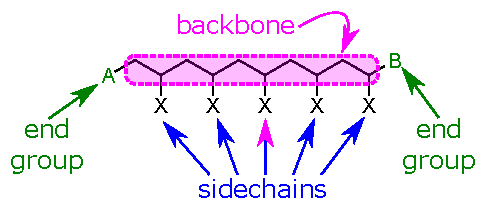
\includegraphics[width=0.5\textwidth]{\figpath/Model1_schematic.pdf}}

\end{model}


\begin{ctqs}

	\question Which of these components (backbone, sidechains, or end groups)...
	
		\begin{enumerate}
			\item ... contain the bonds and/or functional groups that make up the ``main chain'' that spans from one end of the polymer to the other?
			
				\begin{solution}[0.25in]{}
					backbone
				\end{solution}
			
			\item ... contain the functional groups that are attached to every repeat unit but are not part of unbroken string of bonds connecting one end of the polymer to the other?
			
				\begin{solution}[0.25in]{}
					sidechains
				\end{solution}
			
			\item ... ``cap'' the ends of the polymer chain?
			
				\begin{solution}[0.25in]{}
					end groups
				\end{solution}
				
		\end{enumerate}
		
	\question The structure of a polystyrene chain is given below:
	
		\vspace{6pt}
		\centerline{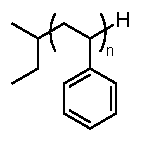
\includegraphics[width=0.15\textwidth]{\figpath/Model1_PS}}
	
		For this polymer, identify and sketch the structures of...
		\begin{enumerate}
			\item the backbone:
			
				\begin{solution}[1in]{}
					The backbone contains the string of C-C bonds highlighted below:
					
					\centerline{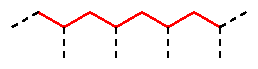
\includegraphics[width=0.3\textwidth]{\figpath/Model1_PS_backbone_soln}}
				\end{solution}
			
			\item the sidechains:
			
				\begin{solution}[0.5in]{}
					The sidechains consist of the aromatic rings, as highlighted below:
					
					\centerline{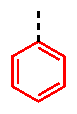
\includegraphics[width=0.075\textwidth]{\figpath/Model1_PS_sidechain_soln}}
				\end{solution}
			
			\item the end groups:
			
				\begin{solution}[0.5in]{}
					The end groups are a sec-butyl group (left) and a hydrogen atom (right), as indicated below:
					
					\centerline{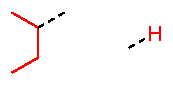
\includegraphics[width=0.2\textwidth]{\figpath/Model1_PS_endgrps_soln}}
				\end{solution}
			
			
		\end{enumerate}
		
	\question Polystyrene is produced from the styrene monomer,
	
		\centerline{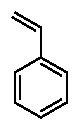
\includegraphics[width=0.1\textwidth]{\figpath/Model1_styrene}}
	
		\begin{enumerate}
			\item Upon polymerization, which bond from this monomer is incorporated into the backbone of the polymer chain?
			
				\begin{solution}[0.5in]{}
				
					The double bond that is not part of the aromatic ring (the vinyl group) is converted to a single bond and incorporated into the backbone of the chain.
					
				\end{solution}
				
			\item How is the structure of the repeat unit related to the structure of this monomer?
			
				\begin{solution}[0.5in]{}
				
					They have the same chemical formula and connectivity of the atoms, but the double bond in the monomer is replaced by a single bond in the polymer, and new bonds are formed to connect the monomer to the adjacent repeat units.
					
				\end{solution}
				
			\item How is the name of the polymer related to the name of this monomer?
			
				\begin{solution}[0.75in]{}
				
					The name of the polymer is just poly( name of the monomer ).
					
				\end{solution}
				
		\end{enumerate}
		
	\question Two other common polymers, and the monomers used to produce them, are shown below:
	
		\centerline{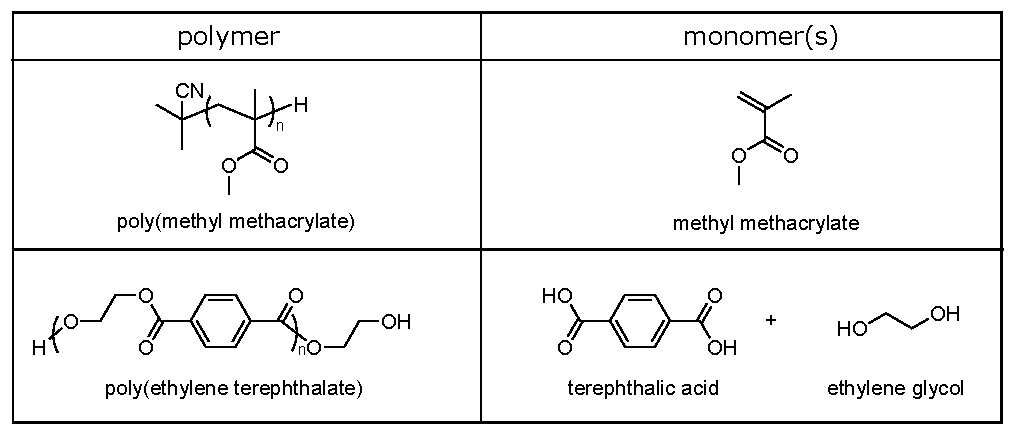
\includegraphics[width=0.8\textwidth]{\figpath/Model1_polymermonomertable}}
		
		Based on these structures, critique or defend each of the following statements in 2-3 complete sentences:
		
		\begin{enumerate}
			\item \emph{``Polymer chains always have backbones consisting of only C-C single bonds.''}
			
				\begin{solution}[1.5in]{}
					This statement is false.  As shown in the table, the backbone of poly(ethylene terephthalate) contains both C-O bonds and C=C bonds (in the aromatic ring) in the chain of bonds connecting one end of the repeat unit to the next.
				\end{solution}
			
			\item \emph{``Polymers are always named for the monomer from which they are produced.''}
			
				\begin{solution}[1.5in]{}
					This statement is also false.  Poly(ethylene terephthalate) is made from terephthalic acid and ethylene glycol, but is not named after either of these monomers individually.
				\end{solution}
			
		\end{enumerate}

\end{ctqs}

\begin{infobox}
	Polymers are typically named for their ``constituent repeat unit.''
\end{infobox}

\begin{ctqs}

	\question The structure of ethylene terephthalate is shown below:
	
		\centerline{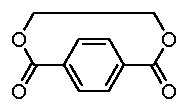
\includegraphics[width=0.2\textwidth]{\figpath/Model1_ethyleneterephthalate}}
		
		Is this structure consistent with the rule given in the above information box?  Briefly explain your group's reasoning.
		
		\begin{solution}[0.75in]{}
			Yes, it is.  This molecule has the same structure as the repeat unit of the poly(ethylene terephthalate) molecule, with only one bond needing to be broken/re-formed to link to adjacent repeat units.
			
			Note that IUPAC specifies clear rules for how the constituent repeat unit is named, which the above examples do not follow - we have given the ``common names'' for the repeat units rather than their IUPAC names.  See DOI 10.1351/PAC-REP-12-03-05 for a brief guide to IUPAC nomenclature.
			
		\end{solution}

\end{ctqs}


\clearpage


\begin{model}[Composition]
\label{\labelbase:mdl:composition}

	Most of the polymers shown in Model \ref{\labelbase:mdl:backsideend} contain only one type of monomer.  However, polymers often contain multiple types of monomers.  The resulting polymers are classified both in terms of how many distinct monomers they contain, and how those monomers are distributed throughout the chain.
	
	Several common classes of polymers are illustrated below:
	
	{\renewcommand{\arraystretch}{1.75}
	\begin{tabular}{m{0.78in}m{2in}m{2.5in}}
		\hline
		Classification & Monomer Distribution & Example\\
		\hline
		Homopolymer & AAAAAAAAAAAAAAAAAA & 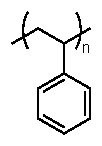
\includegraphics[width=0.4in]{\figpath/Model2_PS} ~~ poly(styrene) \\\hline
		Statistical Copolymer & ABBBABAABBAAAABBAB & 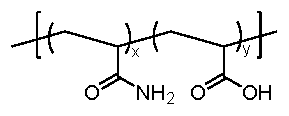
\includegraphics[width=1.25in]{\figpath/Model2_PAmAA} \newline poly(acrylamide-\emph{stat}-acrylic acid)\\\hline
		Alternating Copolymer & ABABABABABABABABAB & 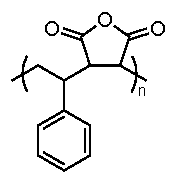
\includegraphics[width=0.75in]{\figpath/Model2_PSaltMA} \newline poly(styrene-\emph{alt}-maleic anhydride)\\\hline
		Diblock Copolymer & AAAAAAAAABBBBBBBBB & 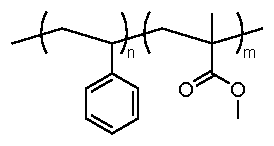
\includegraphics[width=1.25in]{\figpath/Model2_PSblockPMMA} \newline poly(styrene)-\emph{block}-poly(methyl methacrylate)\\\hline
		Triblock Copolymer & AAAAAABBBBBBAAAAAA & 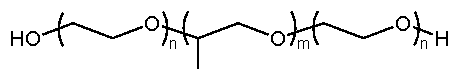
\includegraphics[width=2in]{\figpath/Model2_pluronic} \newline poly(ethylene oxide)-\emph{block}-poly(propyl\-ene oxide)-\emph{block}-poly(ethylene oxide) \\\hline
		Statistical Terpolymer & ABBCABACCCBCAABACB & 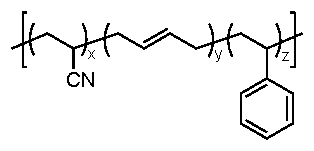
\includegraphics[width=1.5in]{\figpath/Model2_ABS} \newline poly(acrylonitrile-\emph{stat}-butadiene-\emph{stat}-styrene) \\\hline
		Graft Copolymer & 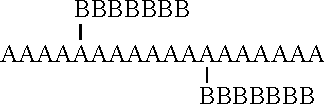
\includegraphics[width=1.75in]{\figpath/Model2_graftschematic} & 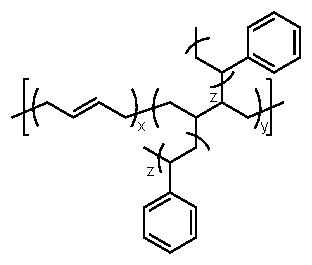
\includegraphics[width=1.25in]{\figpath/Model2_PBgPS} \newline poly(butadiene)-\emph{graft}-poly(styrene) 
	\end{tabular}
	}

\end{model}

\begin{ctqs}

	\question How many types of monomers are included in...
	
		\begin{enumerate}
			\item ... homopolymers?
			
				\begin{solution}[0.25in]{}
				1
				\end{solution}
			
			\item ... copolymers?
			
				\begin{solution}[0.25in]{}
				2
				\end{solution}
			
			\item ... terpolymers?
			
				\begin{solution}[0.25in]{}
				3
				\end{solution}
			
		\end{enumerate}

	\question Describe, in your own words, how the monomers are arranged in...
	
		\begin{enumerate}
			
			\item ... alternating copolymers
			
				\begin{solution}[0.25in]{}
				The monomers alternate between A's and B's (A is always followed by B and vice versa)
				\end{solution}
			
			\item ... block copolymers
			
				\begin{solution}[0.25in]{}
				The A monomers and B monomers are grouped together (all of the A's come first, followed by all of the B's)
				\end{solution}
				
			\item ... statistical copolymers
			
				\begin{solution}[0.25in]{}
				The monomers appear to be randomly distributed along the chain (note: Activity 6.1 will teach students why we refer to ``statistical'' rather than ``random'' copolymers, but random is ok for this question).
				\end{solution}
				
		\end{enumerate}
		
	\item The sequences of alternating, block, and statistical copolymers are reflected by the placement of the parentheses in the skeletal structures of the polymers.
	
		\begin{enumerate}
		
			\item Alternating copolymers can be described as a repeating sequence of (AB) repeat units.  How is this reflected in the placement of the parentheses in the example structure shown in the table?
			
				\begin{solution}[1in]{}
				The structure of the alternating copolymer contains only one set of parentheses.  In the example shown, this set of parentheses surrounds the entire repeat unit containing \emph{both} the styrene monomer \emph{and} the maleic anhydride monomer, indicating that it is this unit containing both monomers in sequence that repeats throughout the polymer chain.
				\end{solution}
			
			\item Block copolymers can be described as an (A) homopolymer connected end-to-end to a (B) homopolymer.  How is this reflected in the placement of the parentheses in the example structure shown in table?  
			
				\begin{solution}[1in]{}
				The structure of the block copolymer contains two sets of parentheses.  In the example shown, the first set surrounds the styrene repeat unit, indicating that there is a repeating homopolymer-like chain of styrene units.  The second set then surrounds only the methyl methacrylate unit, indicating that there is a repeating homopolymer-like chain of methyl methacrylates.  The structures in the two sets of parentheses are joined by a single C-C bond, indicating that the end of the poly(styrene) chain is connected to the end of the poly(methyl methacrylate) chain.
				\end{solution}

			\item What additional feature is present in the skeletal structure of the statistical polymer to indicate that the repeat units are more randomly distributed?
			
				\begin{solution}[1in]{}
				The structure of the statistical copolymer looks like that of the diblock copolymer, but contains an extra set of square brackets outside the parentheses.  The subscripts on the repeat units also change from ``n'' and ``m'' (indicating numbers of repeat units) to ``x'' and ``y'' (indicating fraction of repeat units).
				\end{solution}
			
			\item Summarize, in 2-3 complete sentences, how placement of the parentheses is used to indicate the type of monomer sequence present in a polymer.
			
				\begin{solution}[2in]{}
				For alternating copolymers, a single set of parentheses should be placed around the entire (AB) repeat unit.  For block copolymers, one set of parentheses should be used for each block, and a covalent bond crossing from one set of parenthese to the next indicates the bond between the blocks.  Finally, for statistical copolymers, an extra set of square brackets should be added to indicate the random distribution.
				\end{solution}
			
		\end{enumerate}
	
	\question For block copolymers, which part of the classification name indicates the number of polymer ``blocks''?
			
				\begin{solution}[0.5in]{}
				The prefix on the word ``block'' (``di'' means 2, ``tri'' means 3, etc.) 
				\end{solution}
		
	\question Using the rules you identified above, classify each of the following polymers: 
	
		(\emph{Challenge: if you have extra time, see if you can propose a formal name for each structure, too!})
	
		\begin{enumerate}
			\item \text{}\\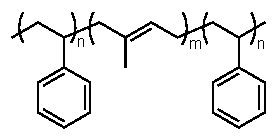
\includegraphics[width=0.25\textwidth]{\figpath/Model2_SBS}
			
				\begin{solution}[0.25in]{}
					triblock copolymer (poly(styrene)-\emph{block}-poly(isoprene)-\emph{block}-poly(styrene))
				\end{solution}
			
			\item \text{}\\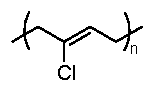
\includegraphics[width=0.15\textwidth]{\figpath/Model2_neoprene}
			
				\begin{solution}[0.25in]{}
					homopolymer (poly(chloroprene))
				\end{solution}
			
			\item \text{}\\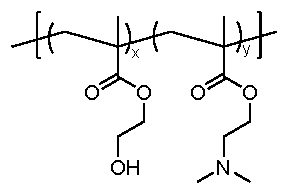
\includegraphics[width=0.2\textwidth]{\figpath/Model2_HEMAstatDMAEMA}
			
				\begin{solution}[0.25in]{}
					statistical copolymer (poly(hydroxyethyl methacrylate - \emph{stat} - dimethylaminoethyl methacrylate))
				\end{solution}
			
		\end{enumerate}
		
	\question Propose a possible sequence of a triblock terpolymer consisting of repeat units A, B, and C.
	
		\begin{solution}[0.25in]{}
		
			AAAAAAAABBBBBBBBBBBBCCCCCCCCCCCCCCCCC
			
			(note: the blocks don't have to be equal lengths or molecular weights!)
	
		\end{solution}
	
	\question Draw the skeletal structure of a statistical copolymer of styrene and acrylonitrile.
	
		\begin{solution}[0.75in]{}
			\centerline{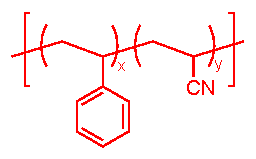
\includegraphics[width=0.25\textwidth]{\figpath/Model2_PSsPAN_soln}}
		\end{solution}
	
\end{ctqs}


%\clearpage
\begin{model}[Isomerism]

	Even when polymers consist of only a single monomer, sometimes that monomer can be incorporated into the polymer chain in different ways.  This results in \textit{isomerism} in the polymer chain.  Three common types of isomerism are illustrated below:
	
	\begin{enumerate}
		\item Positional isomerism:
		
			\centerline{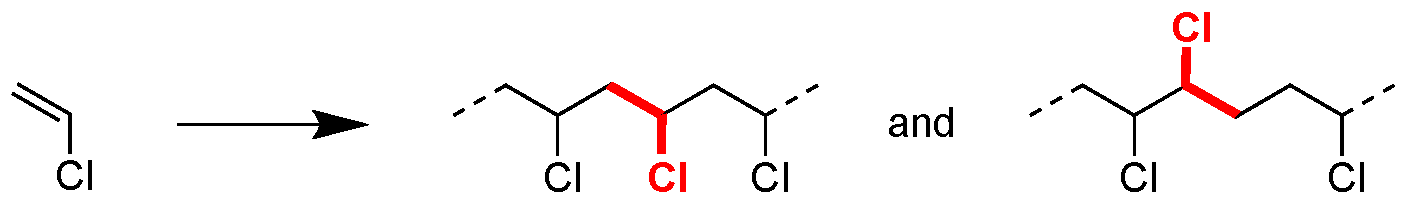
\includegraphics[width=0.7\textwidth]{\figpath/Model3_positional}}
		
		\item Stereoisomerism:
		
			\centerline{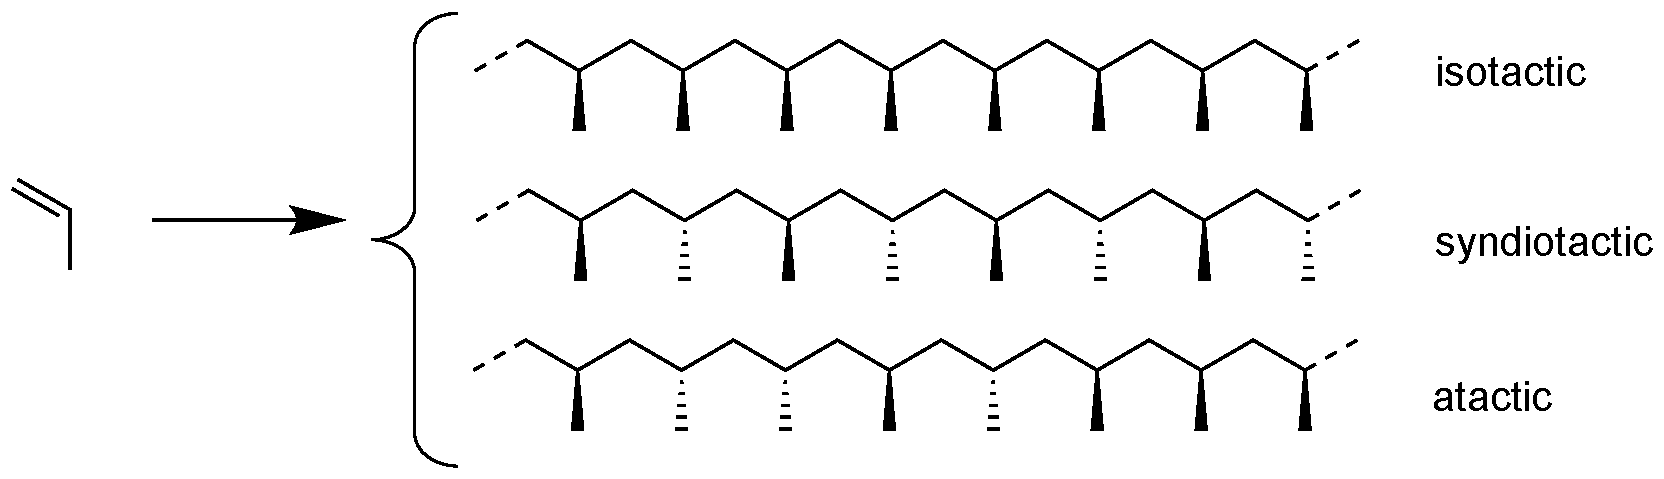
\includegraphics[width=0.8\textwidth]{\figpath/Model3_stereo}}
		
		\item Geometric isomerism:
		
		\vspace{4pt}	\centerline{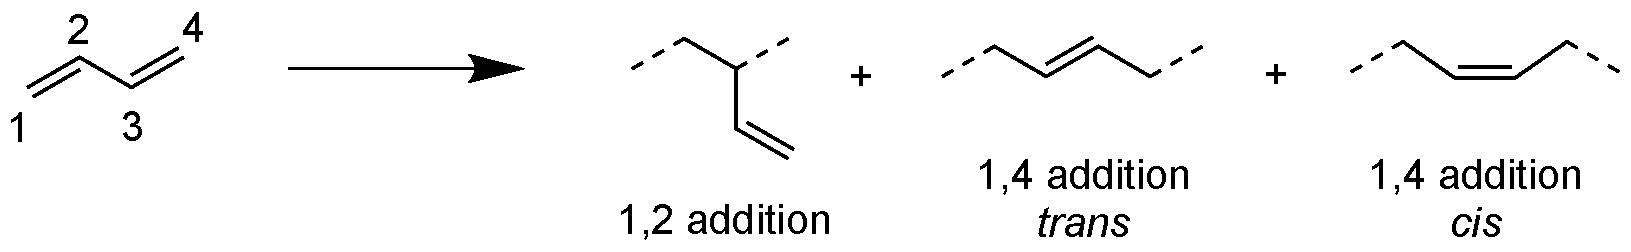
\includegraphics[width=0.8\textwidth]{\figpath/Model3_geometric}}
		
	\end{enumerate}

\end{model}

\begin{ctqs}

	\question What is the primary feature of the polymer chain that differs between...
	
		\begin{enumerate}
			\item ... different \emph{positional} isomers of the same monomer?
			
				\begin{solution}[0.5in]{}
					Positional isomers differ in how the monomer is ``oriented'' within the chain (e.g. whether the sidechain is on the left or right)
				\end{solution}
			
			\item ... different \emph{stereoisomers} of the same monomer?
			
				\begin{solution}[0.5in]{}
					Stereoisomers differ in the relative arrangement of the stereocenters along the polymer backbone
				\end{solution}
			
			\item ... different \emph{geometric} isomers of the same monomer?
			
				\begin{solution}[0.5in]{}
					Geometric isomers differ the bonding patterns of the monomers (including both which bonds are part of the backbone, and the cis/trans isomerization of the double bond).
					
					Note: in discussion, it may be useful to note that 1,2-type addition for butadiene and isoprene is also referred to as ``vinyl''-type addition. 
				\end{solution}
			
		\end{enumerate}
		
	\question Sketch each of the following:
	
		\begin{enumerate}
			\item An 8 repeat-unit segment of syndiotactic poly(acrylonitrile):
			
				\begin{solution}[1in]{}
			\centerline{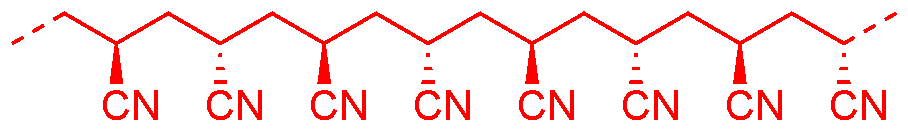
\includegraphics[width=0.45\textwidth]{\figpath/Model3_syndioPAN_soln}}
		\end{solution}
			
			\item The skeletal structure of a statistical copolymer of \emph{cis}-1,4 and \emph{trans}-1,4 polybutadiene:
			
				\begin{solution}[1in]{}
			\centerline{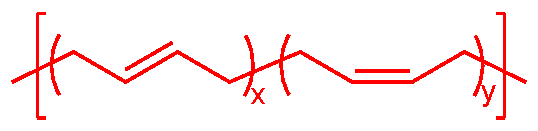
\includegraphics[width=0.35\textwidth]{\figpath/Model3_butadiene_soln}}
		\end{solution}
				
		\end{enumerate}
	
\end{ctqs}


\clearpage
\begin{exercises}

	%\exercise Poly(styrene) is an example of a ``vinyl-type'' polymer.  Vinyl-type polymers have the following general structure, as shown in Model \ref{\labelbase:mdl:backsideend}:
	
	%	IMAGE
		
	%	\begin{enumerate}
		
	%		\item Propose the structure of the monomer that is most likely used to produce this polymer.
			
	%			\emph{Hint: try replacing the aromatic ring in the structures shown in CTQs nnn and mmm with an ``X''!}
			
	%		\item Based on the structure you drew, explain, in 1-2 complete sentences, why these polymers are reasonably described as ``vinyl-type'' polymers.
			
	%	\end{enumerate}
		
	%\exercise Something about IUPAC nomenclature: 10.1351/PAC-REP-12-03-05
		
	%\exercise structure of kraton rubbers (SBS triblocks that then get hydrogenated?)
	
	%\exercise something about random vs statistical copolymers?
		
	\exercise The polymers shown in this activity were (almost) all \emph{linear} polymers, in which the backbone makes a single unbroken line from one end of the molecule to the other.  However, the backbone can also have more complex \emph{architectures}, some of which are illustrated below:
	
	\vspace{6pt}	\centerline{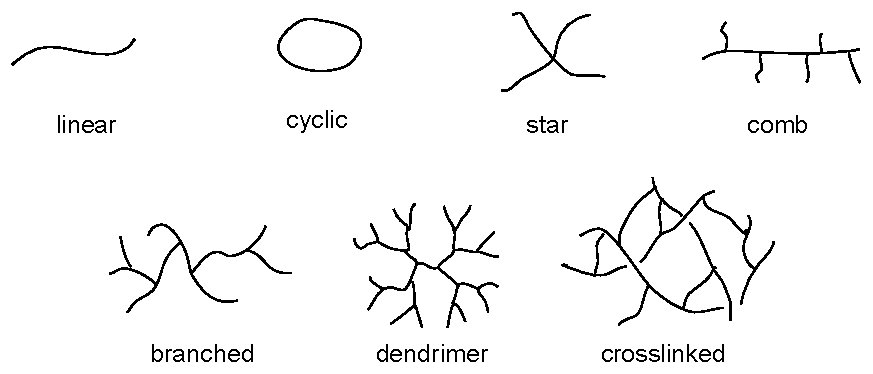
\includegraphics[width=0.6\textwidth]{\figpath/Exc_architectures}}
	
		Identify the architecture that most closely corresponds to each of the following chemical structures:
		
		\begin{enumerate}
			\item \text{}\\ 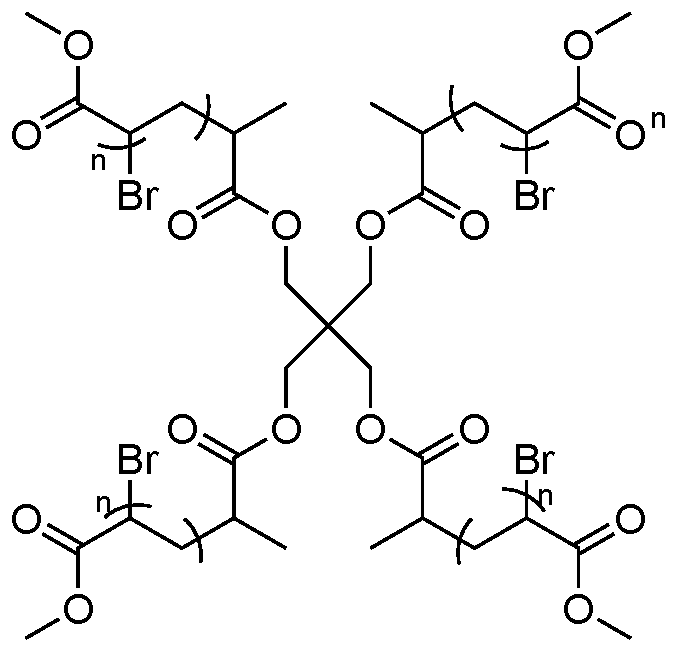
\includegraphics[width=0.25\textwidth]{\figpath/Exc_architectures_star}
			
				\begin{solution}{}
					This structure is a \emph{star} polymer.  4 polymer chains emanate out from a central core.
					
					(If students have trouble seeing this, encourage them to replace each set of bonds between repeat unit parentheses with a wiggly line representing the backbone chain.)
				\end{solution}
			
			\item \text{}\\ 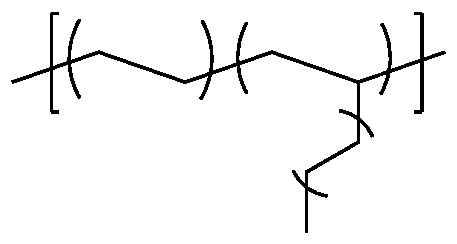
\includegraphics[width=0.2\textwidth]{\figpath/Exc_architectures_comb}
			
				\begin{solution}{}
					This structure is a \emph{comb} polymer.  Poly(ethylene) chains are grafted off of some of the repeat units on a poly(ethylene) backbone.
				\end{solution}
			
			\item \text{}\\ 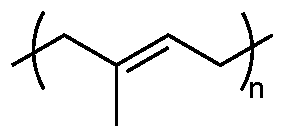
\includegraphics[width=0.15\textwidth]{\figpath/Exc_architectures_linear}
			
				\begin{solution}{}
					This structure is a \emph{linear} polymer.  
					
					Note that some students may determine that this is a comb polymer, because the methyl group in the sidechain looks like the comb structure.  Remind them that in the architectures shown in the problem, the lines refer to the polymer backbone, not the sidechains - there are no \emph{polymer} chains hanging off of the backbone so this structure is not a comb.
				\end{solution}
			
			\item \text{}\\ 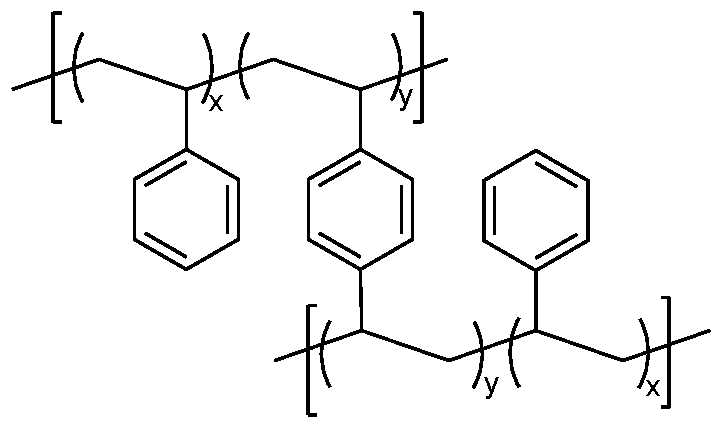
\includegraphics[width=0.3\textwidth]{\figpath/Exc_architectures_xlinked}
			
				\begin{solution}{}
					This structure is a \emph{crosslinked} polymer.  Linear chains are linked by chemical crosslinkers at random locations in the chain(s).
				\end{solution}
			
		\end{enumerate}
	
\end{exercises}

	
\end{activity}